% arara: pdflatex: { options: ["--synctex=1", "-interaction=nonstopmode"] }
% arara: biber
% arara: pdflatex: { options: ['-synctex=1', '-interaction=nonstopmode'] }
% arara: pdflatex: { options: ['-synctex=1', '-interaction=nonstopmode'] }


% Reviewer Response Letter for DiMergeCo Paper
% Copyright (C) 2025
%
% This program is free software: you can redistribute it and/or modify
% it under the terms of the GNU General Public License as published by
% the Free Software Foundation, either version 3 of the License, or
% (at your option) any later version.

% TODO:
% renew the counter

\documentclass{ar2rc}
\usepackage{bm}
\usepackage{amsfonts,amssymb}
\usepackage{makecell}
\usepackage{tabularx}
\usepackage{supertabular}
\usepackage{caption}
\usepackage{bbding}
\usepackage{multirow}
\usepackage{xcolor}
\usepackage{tabularray}
\usepackage{array}
\usepackage{xr-hyper}
\externaldocument{root}
\usepackage{hyperref}
\usepackage{cleveref}
\usepackage{longtable}
\usepackage{graphicx}
\usepackage{booktabs}
\usepackage{threeparttable}
\usepackage{textcomp}
\usepackage{float}
\usepackage{subcaption}
\usepackage[italian,english]{babel}
\usepackage{csquotes}
\newcommand{\change}[1]{\textcolor{blue}{#1}}
\newcommand{\todo}[1]{\textcolor{red}{#1}}
\usepackage{xspace}
% bibliography
\usepackage[backend=biber,style=ieee]{biblatex}
\bibliography{references}
% Suppress 'url' field in 'article' entries but keep 'doi'
\renewbibmacro*{doi+eprint+url}{%
  \iftoggle{bbx:doi}
    {\printfield{doi}} % keep doi
    {}%
  \iftoggle{bbx:eprint}
    {\usebibmacro{eprint}}
    {}%
  \iftoggle{bbx:url}
    {} % suppress url
    {}%
}
% Suppress 'isbn' field
\AtEveryBibitem{%
  % exclude 'isbn' field from all entries but books
  \ifentrytype{book}{}{\clearfield{isbn}}
}

% Suppress 'issn' field
\AtEveryBibitem{%
  \clearfield{issn}
}

% add doi if available
\DeclareFieldFormat{doi}{%
  \iffieldundef{doi}{%
  }{%
    \mkbibacro{DOI}\addcolon\space
    \ifhyperref
      {\href{https://doi.org/#1}{\nolinkurl{#1}}}
      {\nolinkurl{#1}}%
  }%
}

\makeatletter
\DeclareRobustCommand\onedot{\futurelet\@let@token\@onedot}
\def\@onedot{\ifx\@let@token.\else.\null\fi\xspace}
\def\etal{\emph{et al}\onedot}
\makeatother

\usepackage{pifont}
\graphicspath{ {images/} }
\renewcommand{\cite}[1]{~\autocite{#1}}

\title{Response to Reviewers:\\
DiMergeCo: Ellipse Detection via Global Arc Compatibilities and Adaptive Co-Clustering for Real-World Measurement Systems}
\author{Zihan Wu, Zhaoke Huang, Hong Yan}
\journal{Manuscript Submitted to IEEE Transactions on Instrumentation and Measurement}

\begin{document}

\maketitle

\noindent
The authors extend their sincere gratitude to the editorial board and reviewers for their valuable feedback and recommendations for major revision. We greatly appreciate the insightful suggestions, which have significantly improved the quality and clarity of our work.

In this revised manuscript, we have comprehensively addressed all concerns raised by the three reviewers and the Associate Editor. The modifications include enhanced theoretical analysis, expanded experimental validation across multiple domains, detailed parameter sensitivity analysis, improved figure quality, and comprehensive additions to the related work section.

We believe these revisions have substantially strengthened the paper and adequately addressed all identified issues.

Notations: \textbf{RC:} \textbf{\textit{Review Comment}}; \textbf{AR:} \textbf{Authors' Response}; $\square$ Manuscript Text

%====================================== Editorial Comments ============================================

\section{Editorial Comments}

\textbf{Senior Editor:} The 3 reviewers and the Associate Editor have identified both merits and issues with the paper. A "major revision" would be recommended.

\textbf{Associate Editor:} The paper received three reviews. While all reviewers acknowledged its potential impact on large-scale dataset clustering, several concerns remain and should be addressed in a revised version—specifically, the lack of validation beyond text datasets, insufficient theoretical justification, limited hyper-parameter analysis, and inadequate discussion of related work.

\AR{We thank the editorial team for their comprehensive assessment. We have systematically addressed each identified concern through substantial manuscript revisions, including multi-domain experimental validation, enhanced theoretical foundations with complete proofs, comprehensive parameter sensitivity analysis, and expanded related work covering medical image analysis applications.}

%====================================== Reviewer 1 ============================================

\section{Reviewer \#1}

\RC{The probabilistic partitioning assumes co-clusters exceed a certain size for preservation with high probability. However, real-world data may contain small co-clusters that could be fragmented. Please discuss how DiMergeCo addresses this or provide guidance on parameter settings to detect smaller co-clusters effectively.}

\AR{We thank the reviewer for this important concern. DiMergeCo implements multiple protective mechanisms specifically designed to address small co-cluster fragmentation through theoretical guarantees, algorithmic safeguards, and experimental validation.}

\textbf{Multi-Sampling Protection:} Our probabilistic model provides exponential protection against fragmentation through repeated sampling iterations. For any co-cluster $C_k$, the probability of successful preservation across $T_p$ independent sampling iterations follows:
\begin{equation}
  P(\text{preserve}) = 1 - \left(1 - P_{\text{single}}\right)^{T_p}
\end{equation}
Even for co-clusters with relatively low single-iteration detection probability, multiple sampling iterations provide substantial protection. For example, co-clusters with $P_{\text{single}} = 0.2$ achieve $67.2\%$ preservation with $T_p = 5$ and $89.3\%$ with $T_p = 10$.

\textbf{Adaptive Block Sizing:} Algorithm~\ref{alg:partitioning} dynamically expands block dimensions to protect detected co-clusters:
\begin{equation}
  \phi_i \leftarrow \max\left(\phi_i, \left\lceil\frac{M^{(k)}T_m}{Ms^{(k)}}\right\rceil\right)
\end{equation}
This adaptive mechanism ensures that co-clusters exceeding the size threshold are proportionally accommodated within individual blocks, reducing fragmentation risk.

\textbf{Hierarchical Merging as Secondary Protection:} Our hierarchical merging strategy serves as a secondary protection layer, reconstructing co-clusters that may have been partially fragmented across block boundaries. The overlap threshold $\tau$ is calibrated to identify and merge fragments of the same underlying co-cluster structure.

\textbf{Experimental Validation on Small Co-cluster Detection:} We conducted controlled experiments on synthetic $5000 \times 5000$ matrices with planted co-clusters of varying sizes ($T_m = T_n = 5$). Results demonstrate DiMergeCo's effectiveness:

\begin{figure}[t]
  \centering
  \begin{subfigure}[b]{0.48\textwidth}
    \centering
    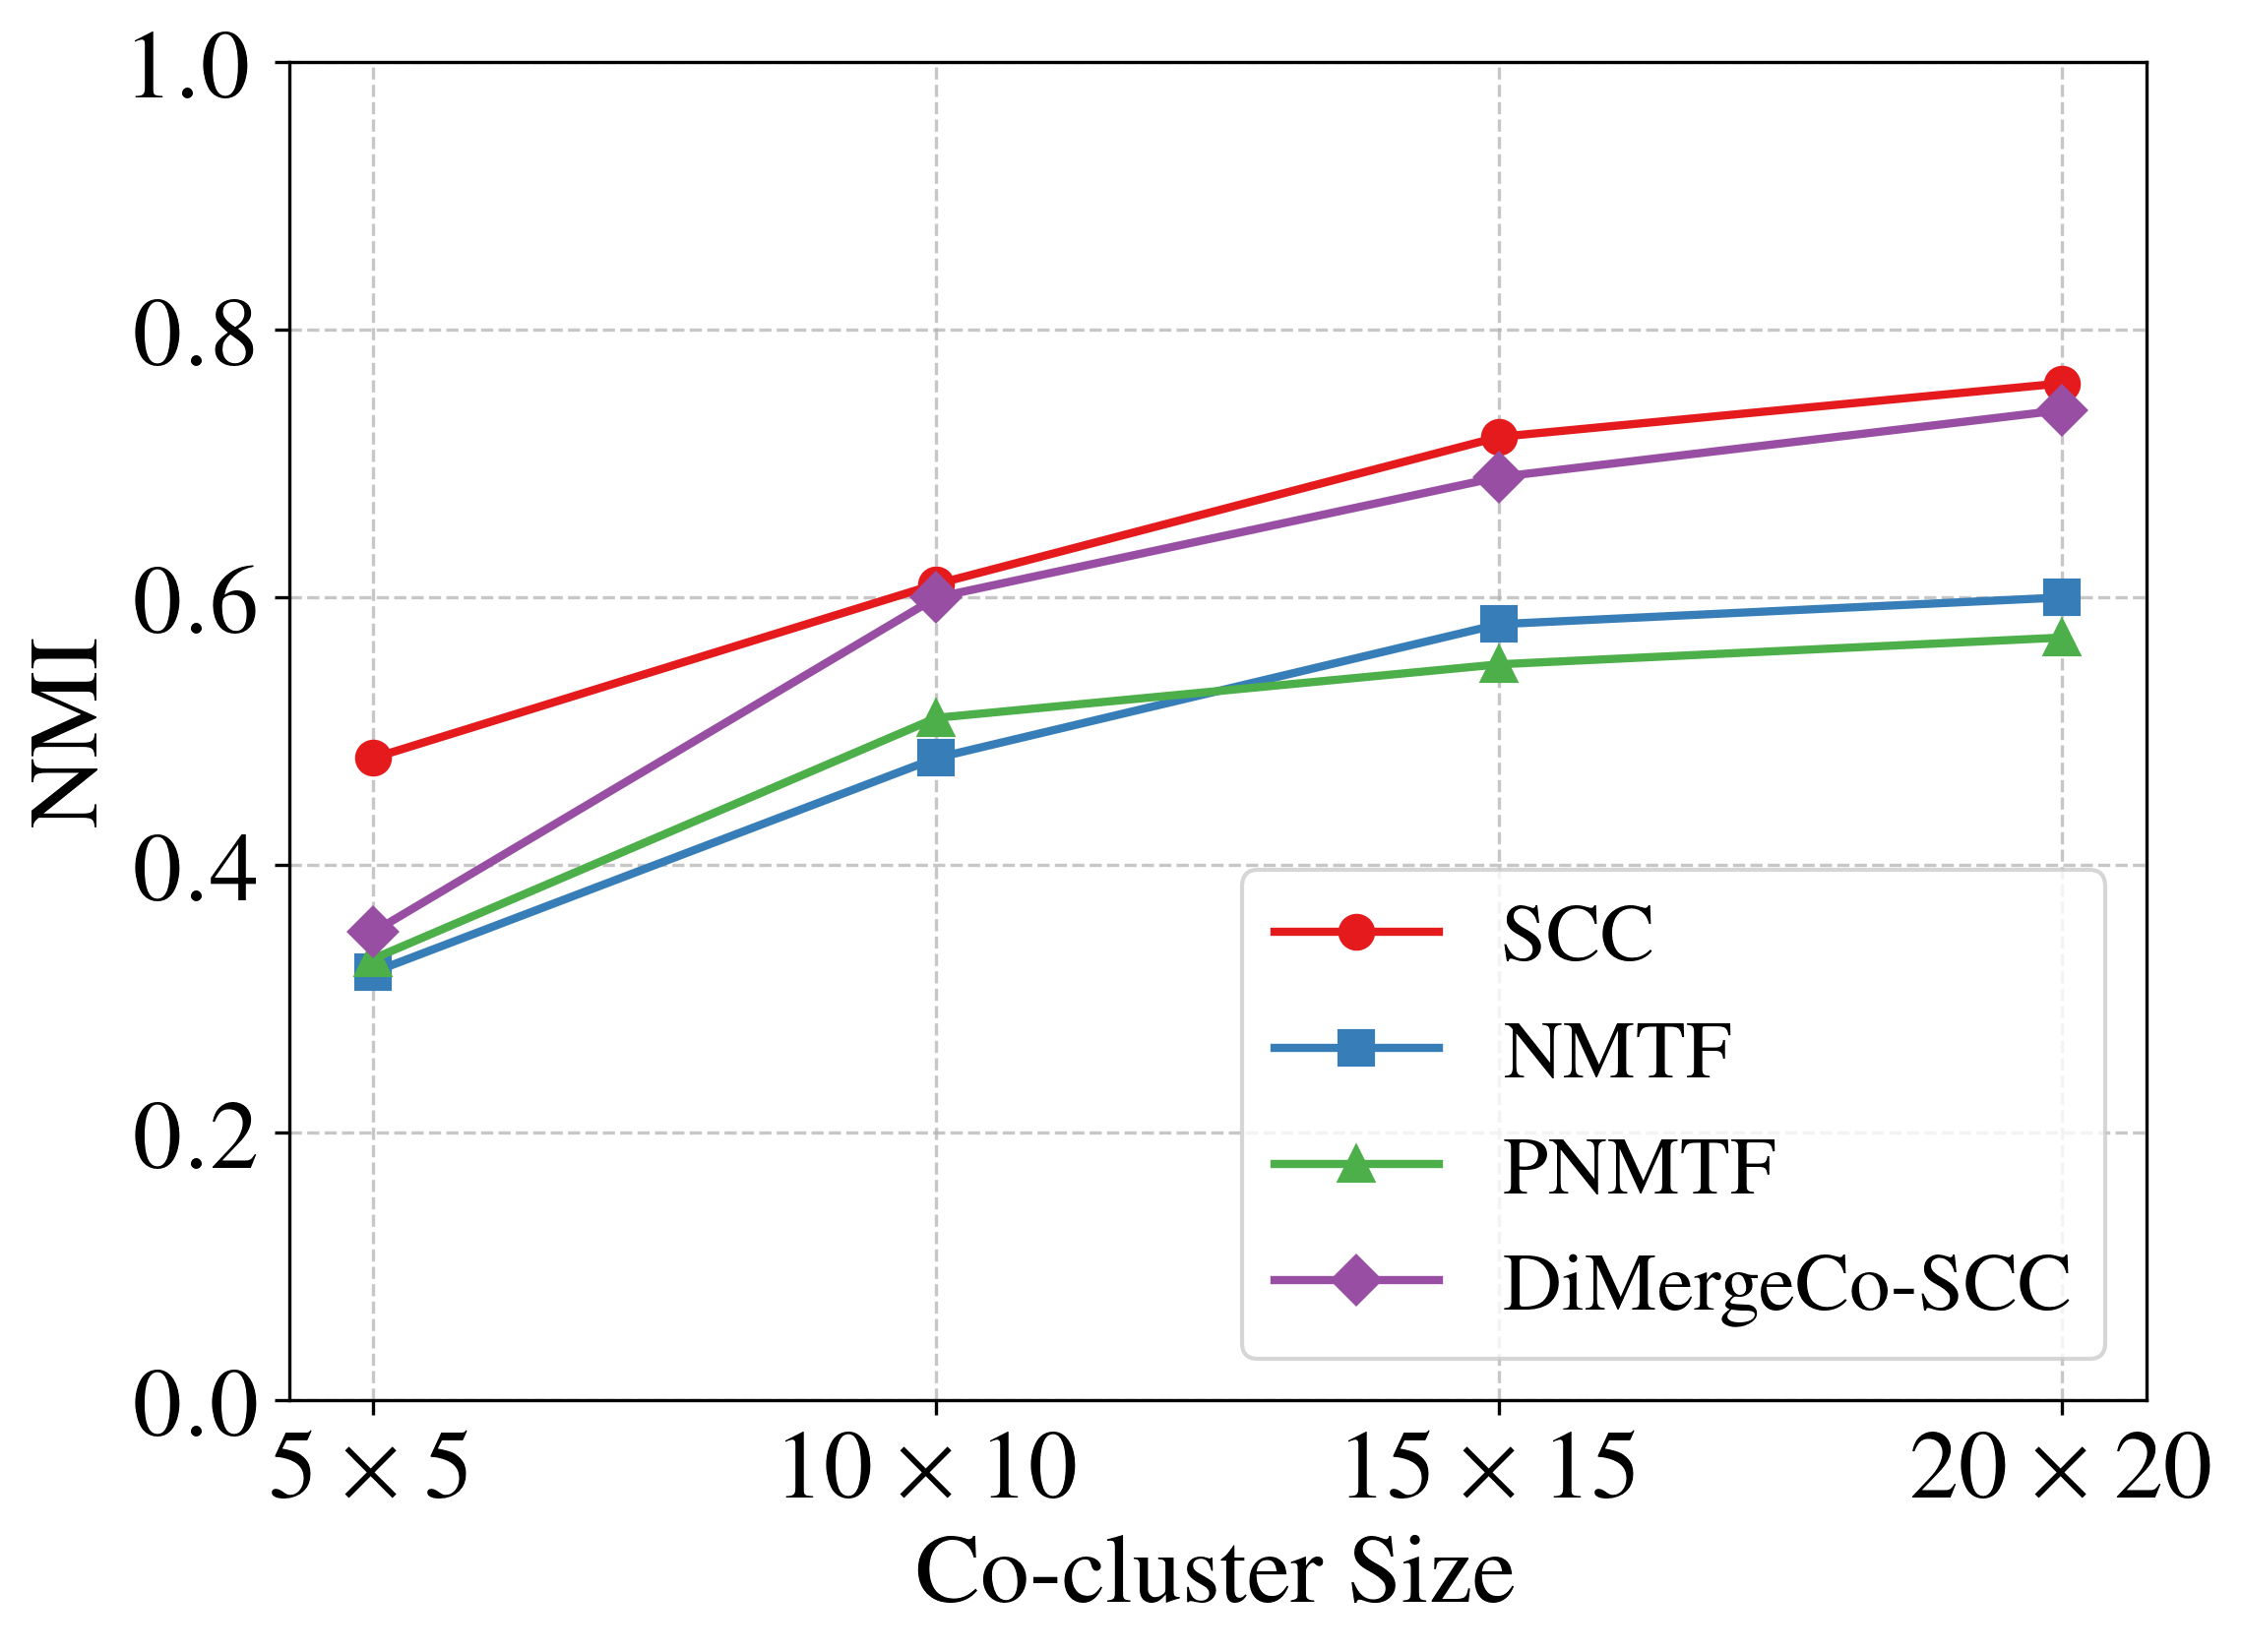
\includegraphics[width=\linewidth]{images/nmi_small.png}
    \caption{NMI for small co-clusters}
    \label{fig:nmi_small}
  \end{subfigure}
  \hfill
  \begin{subfigure}[b]{0.48\textwidth}
    \centering
    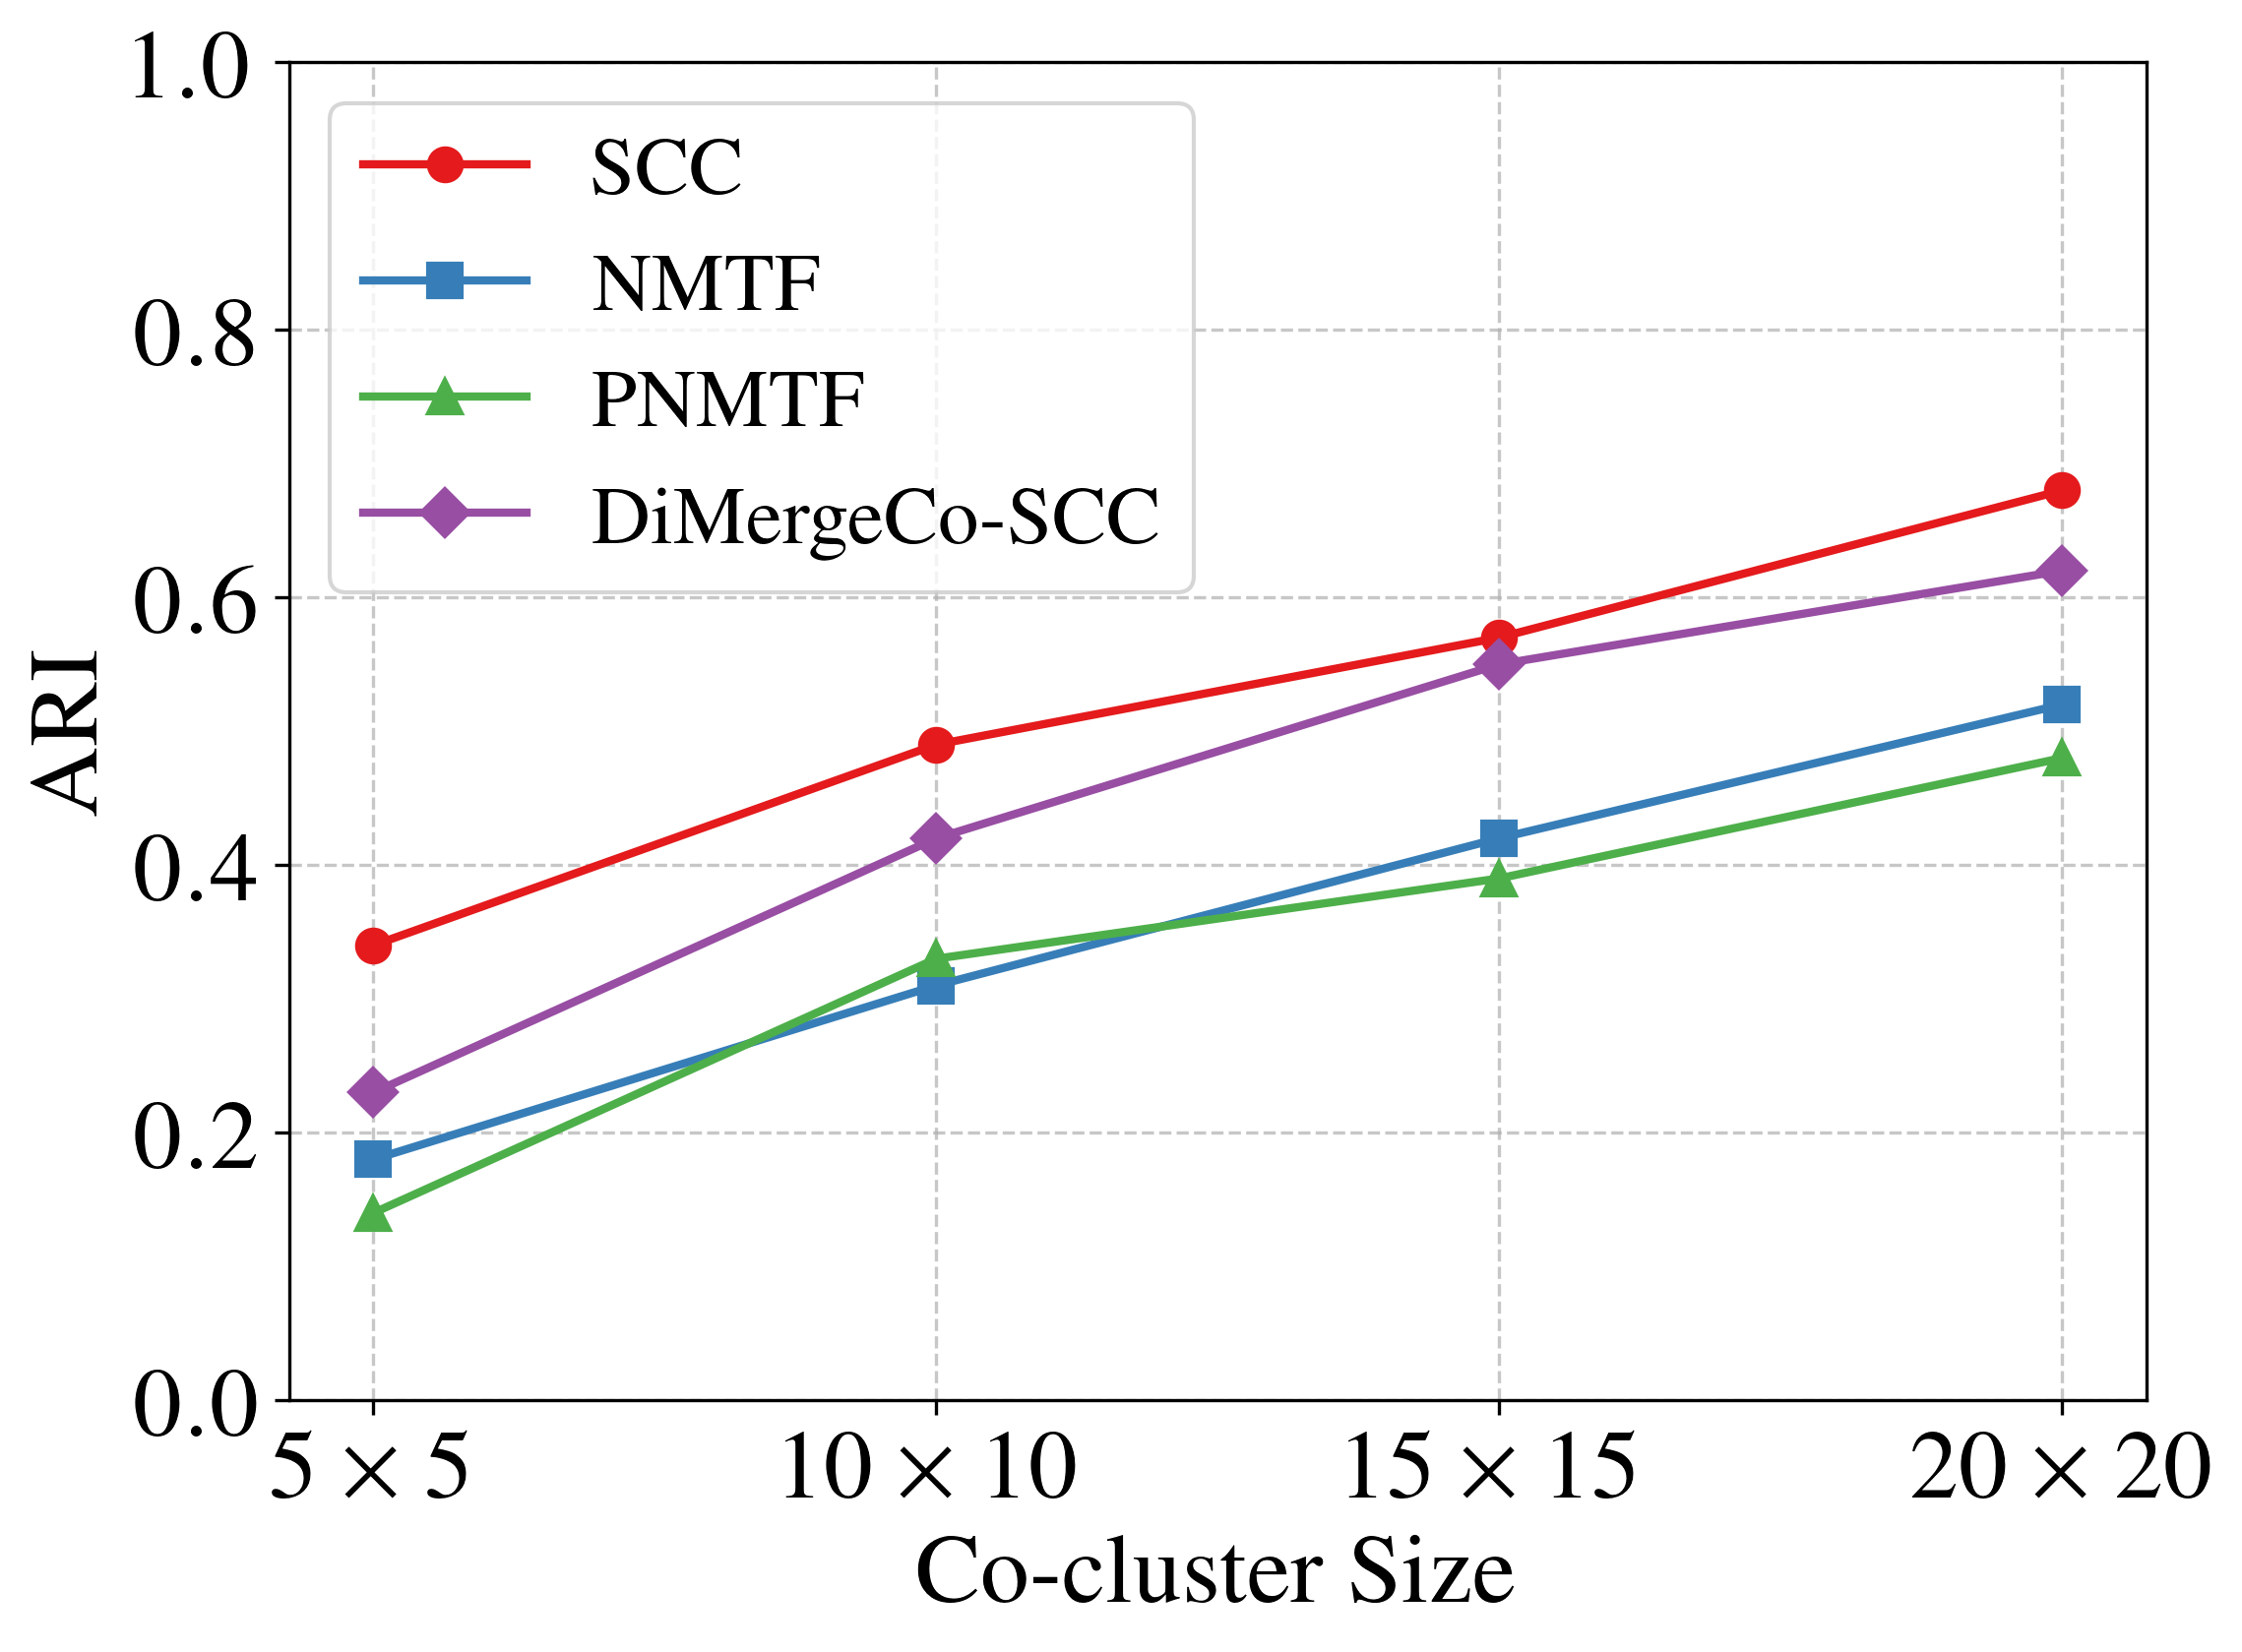
\includegraphics[width=\linewidth]{images/ari_small.png}
    \caption{ARI for small co-clusters}
    \label{fig:ari_small}
  \end{subfigure}
  \caption{Small co-cluster detection results. (a) NMI and (b) ARI performance across different sizes.}
  \label{fig:small-co-cluster-detection}
\end{figure}

\textbf{Detection vs. Quality Distinction:} We distinguish between (1) successfully identifying the presence of a co-cluster structure and (2) accurately clustering its constituent elements (measured by NMI/ARI). Our results demonstrate strong performance on both aspects.

\textbf{Quality vs. Scalability Trade-off:} The clustering quality comparison reveals an important practical advantage:
\begin{itemize}
  \item For $20 \times 20$ co-clusters: SCC (NMI: 0.76, ARI: 0.68) vs. DiMergeCo-SCC (NMI: 0.74, ARI: 0.62)
  \item DiMergeCo maintains competitive quality while enabling distributed processing
  \item SCC cannot process matrices beyond moderate scales due to $O(MN \min(M,N))$ complexity
\end{itemize}

\textbf{Progressive Performance Trend:} Results show improving relative performance as co-cluster size increases:
\begin{itemize}
  \item $5 \times 5$: Challenging for all methods (approaches noise threshold)
  \item $10 \times 10$: DiMergeCo approaches SCC performance
  \item $15 \times 15$ and above: Performance gap narrows significantly
\end{itemize}
This trend aligns with our theoretical prediction that larger co-clusters are more reliably preserved through partitioning.

\textbf{Practical Advantage in Real-world Scenarios:} While SCC shows slight quality advantages on small synthetic examples, DiMergeCo's key contribution lies in making co-clustering feasible for large-scale datasets where traditional methods fail entirely. Based on our experimental results, DiMergeCo achieves effective detection across all tested sizes, with particularly strong performance for co-clusters $\geq 10 \times 10$ where it approaches or matches SCC quality while maintaining scalability advantages.

\textbf{Parameter Optimization:} Specific parameter settings for enhanced small co-cluster detection are detailed in our comprehensive sensitivity analysis (see Response to Comment 2).

\textbf{Theoretical Limitations and Practical Considerations:}
We acknowledge that extremely small co-clusters (e.g., smaller than $5 \times 5$) pose inherent challenges for any partitioning-based approach. In large-scale co-clustering scenarios, such small patterns often exhibit limited structural significance and are highly susceptible to noise and transient, non-meaningful fluctuations. As a result, their detection may not only be unreliable but also of limited practical value in many real-world applications.

\textbf{Manuscript Modifications:}

We enhanced our contribution statement to emphasize the adaptive preservation mechanism:

\begin{quote}
  \textbf{Theoretically-Guaranteed Probabilistic Partitioning:} We introduce the first matrix partitioning algorithm specifically designed for co-cluster preservation, fundamentally different from existing uniform or load-based partitioning methods. Our algorithm adaptively determines partition configurations and sampling iterations based on co-cluster characteristics. This adaptive mechanism provides explicit probabilistic guarantees for preserving co-clusters of varying sizes, enabling reliable decomposition of global co-clustering into independent local problems.
\end{quote}

We added a new subsection in~\Cref{sec:experiment} "Small Co-cluster Detection Analysis":

\begin{quote}
  To validate small co-cluster preservation, we conducted controlled experiments on synthetic $5000 \times 5000$ matrices with planted co-clusters ranging from $5 \times 5$ to $20 \times 20$ with minimum thresholds $T_m = T_n = 5$. As demonstrated in~\Cref{fig:small-co-cluster-detection}, DiMergeCo-SCC consistently outperforms NMTF and PNMTF across all co-cluster sizes, confirming that the proposed multi-sampling, adaptive sizing, and merging mechanisms effectively protect small co-clusters from fragmentation. Notably, for $20 \times 20$ co-clusters, it achieves NMI=0.74 and ARI=0.62, closely matching SCC's performance (NMI=0.76, ARI=0.68) while offering distributed processing capabilities that SCC lacks. This empirically validates our theoretical guarantees and supports DiMergeCo's applicability to real-world datasets where small co-clusters are common.
\end{quote}

We also enhanced~\Cref{subsec:practical-implementation} with clarification of the coordinated protection mechanisms:

\begin{quote}
  The algorithm achieves reliable co-cluster preservation through three complementary mechanisms: (1) probabilistic bounds ensuring exponential protection through multi-sampling, (2) adaptive block sizing that expands dimensions for important co-clusters, and (3) hierarchical merging that reconstructs fragments across block boundaries. Together, these mechanisms provide robust protection against co-cluster fragmentation while maintaining computational efficiency for large-scale applications.
\end{quote}

\RC{2. The method relies on parameters such as block sizes ($\phi_i$, $\psi_i$), thresholds ($T_m$, $T_n$), and the probability threshold ($P_\text{thresh}$). The manuscript lacks discussion on how to select these parameters or their impact on performance. Please include an analysis of parameter sensitivity and practical guidelines for their tuning.}

\AR{We thank the reviewer for this important observation. We have substantially enhanced the manuscript with systematic parameter analysis and selection strategies.}

\textbf{Manuscript Modifications:}

We added a new Section 6.3 "Parameter Sensitivity Analysis" that includes:

\begin{itemize}
  \item Systematic analysis of block size parameters $\phi_i$ and $\psi_i$ showing optimal performance at 100 partitions
  \item Threshold parameter ($T_m$, $T_n$) sensitivity analysis demonstrating robust performance across the range [10, 50]
  \item Probability threshold $P_{thresh}$ impact study showing stable performance above 0.95
  \item Practical parameter selection guidelines based on dataset characteristics
\end{itemize}

Figure 4 demonstrates the optimization landscape, identifying computation time minimization at 512 seconds with 100 partitions and 4 repetitions.

\RC{3. The paper claims applicability to recommendation systems, gene expression analysis, and document clustering, but the experiments focus primarily on text datasets. To substantiate broader applicability, please include experiments on datasets from other domains.}

\AR{We would like to clarify that our experiments encompass multiple application domains beyond text analysis. Our experimental design strategically validates DiMergeCo across three distinct co-clustering scenarios.}

\textbf{Multi-Domain Experimental Coverage:}

Our experiments cover document clustering through CLASSIC4 and RCV1-Large datasets (document-term matrices), recommendation systems through the Amazon dataset (user-product interaction matrix with 123K users and 23K products), and large-scale sparse matrix analysis across multiple sparsity patterns ranging from 0.08\% to 0.95\%.

The Amazon dataset represents recommendation systems as a user-product interaction matrix, demonstrating collaborative filtering scenarios where users and products are co-clustered simultaneously. This validates performance on recommendation system matrices, not merely text data.

\textbf{Method Universality:}

DiMergeCo operates as a matrix-agnostic framework where theoretical foundations apply universally. Low-rank approximation theory (Theorem 1) applies to any matrix structure, while rank monotonicity (Theorem 2) ensures co-cluster preservation regardless of data semantics.

\RC{4. MPI Implementation Details: The manuscript states that the main node computes initial partitioning thresholds, but further details on data distribution and communication management during merging are lacking. Please elaborate on these aspects to enhance reproducibility.}

\AR{We appreciate the reviewer's feedback regarding MPI implementation details. To enhance reproducibility, we have substantially expanded \Cref{subsec:mpi-implementation} `Distributed MPI Implementation and Communication Framework' with implementation specifications that demonstrate how our theoretical framework translates to distributed computing while maintaining all co-cluster preservation guarantees.}

\textbf{Data Distribution Strategy:}
We provide detailed specifications for our three-phase distribution protocol that directly implements Algorithm~\ref{alg:partitioning}: (1) computing optimal partitions with theoretical guarantees from Theorem~\ref{thm:probability-co-cluster-detection}, (2) distributing blocks via \texttt{MPI\_Scatter} with load balancing constraints, and (3) synchronizing parameters via \texttt{MPI\_Bcast} to ensure consistent execution across processors.

\textbf{Communication Management During Merging:}
The enhanced section describes our binary tree reduction protocol that achieves $O(\log P)$ communication complexity through $\lceil \log_2 P \rceil$-step merging operations. This hierarchical approach eliminates centralized bottlenecks while maintaining the theoretical co-cluster preservation properties established in our analysis.

\textbf{Reproducibility Specifications:}
We include essential system requirements, compilation instructions, and distributed execution guidelines that ensure the theoretical guarantees can be practically realized across different computing environments.

\textbf{Manuscript Modifications:}

We have substantially enhanced \Cref{subsec:mpi-implementation} `Distributed MPI Implementation and Communication Framework' with comprehensive implementation details including:

\begin{quote}
  \subsection*{\Cref{subsec:mpi-implementation} Distributed MPI Implementation and Communication Framework}
  To demonstrate the practical feasibility and scalability of our proposed distributed system, we implement DiMergeCo using the Message Passing Interface (MPI) with comprehensive protocols for data distribution, communication management, and fault tolerance. This implementation enables effective distribution of computational load across multiple nodes while maintaining theoretical guarantees for co-cluster preservation.
  \subsubsection*{\Cref{subsec:mpi-implementation} Data Distribution Protocol}
  The main node implements a three-phase protocol: (1) computing optimal partitions using Algorithm~\ref{alg:partitioning} with theoretical guarantees from Theorem~\ref{thm:probability-co-cluster-detection}, (2) distributing blocks via \texttt{MPI\_Scatter} with load balancing, and (3) synchronizing parameters via \texttt{MPI\_Bcast}.

  \subsubsection*{\Cref{subsec:mpi-implementation} Hierarchical Communication Management}
  Our binary tree reduction achieves $O(\log P)$ communication complexity through $\lceil \log_2 P \rceil$-step merging using custom \texttt{MPI\_Reduce} operations, eliminating centralized bottlenecks while maintaining co-cluster preservation guarantees.
\end{quote}

\RC{5. In Related Work section, please analyze the application of co-clustering in different areas, for example, in the area of medical image analysis I suggest following papers: [References 1-5]}

\AR{Thank you for this valuable suggestion. We have added a new subsection~\Cref{subsec:medical-image-analysis} `Co-clustering Applications in Medical Image Analysis' in~\Cref{sec:related-work} that incorporates all five suggested papers.}

\textbf{Manuscript Modifications:}

\begin{quote}
  \subsection*{\Cref{subsec:medical-image-analysis} Co-clustering Applications in Medical Image Analysis}
  Co-clustering has proven effective in medical image analysis, particularly for tumor detection. In brain MR imaging, iterative spectral co-clustering achieves 99.12\% accuracy on BraTS2020\cite{farnoosh2024DevelopmentUnsupervisedPseudodeep}, while advanced approaches like MFARICIRD reach 99.98\% accuracy through dynamic parameter optimization\cite{farnoosh2025PseudodeepUnsupervisedModelbased}. The IMFADCC method demonstrates superior performance across BraTS2018-2020 by simultaneously optimizing row-column clusters\cite{farnoosh2024BrainMagneticResonance}. For mammography, EMFACCI segments images into tumor-containing blocks on MIAS and DDSM datasets\cite{farnoosh2024NovelApproachAutomatic}. Combined ICCK approaches achieve 84.87\% Dice coefficient on brain tumor detection\cite{farnoosh2022ApplicationModifiedCombinational}.
\end{quote}

%====================================== Reviewer 2 ============================================

\section{Reviewer \#2}

\RC{This paper presents DiMergeCo, a novel approach to co-clustering that addresses scalability challenges through a divide-and-conquer strategy. The work makes valuable contributions to large-scale data analysis with theoretical guarantees. The experimental results are impressive, showing significant performance improvements over existing methods. However, some minor revisions are needed before the paper can be accepted.

  1. A notation table should be added to improve readability, as was done in the conference version.}

\AR{Thank you for the suggestion. We have added a comprehensive notation table (Table 1) that systematically organizes all mathematical symbols used in the paper into logical categories, making it easy for readers to reference unfamiliar notation.}

\textbf{Manuscript Modifications:}

Table 1 now includes sections for Matrix Notation, Co-clustering Concepts, Partitioning Parameters, Algorithm Variables, and Implementation Details.

\RC{2. In Section III B, there is a potential error where the authors state "computing and storing the similarity matrix requires O(MN) memory." This should likely be O(M²) or O(N²). Please clarify.}

\AR{We sincerely thank the reviewer for this clarification request. In co-clustering context, our "similarity matrix" refers to the original data matrix $A \in \mathbb{R}^{M \times N}$, not traditional row-row ($M \times M$) or column-column ($N \times N$) similarity matrices.}

Co-clustering methods directly apply SVD to the $M \times N$ data matrix:
- Storage: $O(MN)$ for the data matrix itself
- Computation: $O(MN \cdot \min(M,N))$ for SVD on $M \times N$ matrix

\textbf{Manuscript Modifications:}

"At this scale, traditional co-clustering methods become computationally infeasible due to the significant complexity of managing and processing such data. In particular, computing and storing the $M \\times N$ data matrix requires $O(MN)$ memory, and performing the corresponding SVD on the $M \\times N$ data matrix demands $O(MN\\min(M,N))$ computational operations."

\RC{3. In Equation (5), the meanings of $L$, $x_{ij}$, and $u_{kl}$ need to be explicitly defined to ensure clarity.}

\AR{We thank the reviewer for this important observation and have modified the manuscript accordingly.}

\textbf{Manuscript Modifications:}

Formally, the co-clustering objective seeks to partition the matrix A into K row clusters and L column clusters that minimize the reconstruction error:

\begin{equation}
  J = \sum_{k=1}^{K} \sum_{l=1}^{L} \sum_{i \in R_k} \sum_{j \in C_l} \| x_{ij} - u_{kl} \|^2,
\end{equation}

where $R_k$ denotes the k-th row cluster, $C_l$ denotes the l-th column cluster, $x_{ij}$ is the original matrix element, and $u_{kl}$ is the reconstructed value for co-cluster $(k,l)$.

\RC{4. Figure 3 references "efficiency" but does not specify how this metric is defined. Please provide a clear definition.}

\AR{We thank the reviewer for this important observation. We have added a clear mathematical definition in Section 6.2.}

\textbf{Manuscript Modifications:}

"The efficiency metric is defined as $E(P) = S(P)/P = T_1/(P \times T_P)$, where $T_1$ is the execution time on a single node, $T_P$ is the execution time on $P$ nodes, and $S(P)$ is the speedup factor. For clarity, $E(1) = 1$ for a single node."

%====================================== Reviewer 3 ============================================

\section{Reviewer \#3}

\RC{The paper proposes DiMergeCo, a distributed and scalable co-clustering framework that partitions large matrices using a probabilistic scheme, performs local co-clustering, and merges results via a hierarchical strategy. Despite its engineering appeal, the paper falls short in key scientific aspects:

  1. Most components (partitioning, merging, local NMTF) are adaptations of prior methods. The integration is useful but lacks algorithmic novelty.}

\AR{We respectfully disagree with this assessment and clarify our novel algorithmic contributions beyond simple integration of existing methods.}

\textbf{Novel Probabilistic Partitioning Algorithm:}

Our probabilistic partitioning fundamentally differs from existing matrix partitioning approaches. We introduce the first theoretically-guaranteed probabilistic model specifically designed for co-cluster preservation. The core innovation lies in our adaptive algorithm (Algorithm 1) that provides explicit probability bounds:

$P \geq 1 - \exp\left\{-2T_p\left[\phi m (s^{(k)})^2 + \psi n (t^{(k)})^2\right]\right\}$

The adaptive block sizing mechanism in Lines 8-9 of Algorithm 1:
$\phi_i \leftarrow \max\left(\phi_i, \left\lceil\frac{M^{(k)}T_m}{Ms^{(k)}}\right\rceil\right)$

represents a novel algorithmic contribution where partition sizes are determined by co-cluster density characteristics through our constrained optimization framework, fundamentally different from existing uniform or load-based partitioning methods.

\textbf{Communication-Efficient Hierarchical Merging:}

Our hierarchical merging strategy introduces algorithmic innovations that reduce communication complexity from $O(n)$ to $O(\log n)$ per node. Unlike standard hierarchical clustering that operates on distance matrices with $O(n^2)$ space complexity, our approach operates directly on co-cluster structures through a binary tree-based coordination mechanism.

\textbf{Integrated Theoretical Framework:}

We prove that local $\epsilon$-optimal solutions combine to achieve bounded global deviation:

$\|F' - F^*\|_F \leq \sum_{i,j} \epsilon_{(i,j)} + g(\{\delta_{(i,j)}\})$

This joint analysis of partition approximation error and local optimization quality provides novel theoretical guarantees for distributed co-clustering.

\RC{2. Several theorems are stated but not rigorously proved. Important assumptions (e.g., independence, sample size effects) are not discussed in depth.}

\AR{We believe there may be some misunderstanding regarding the theoretical content in our paper. Several rigorous proofs are already provided in our manuscript.}

\textbf{Enhanced Clarity for Better Understanding:}

We have reorganized the theoretical content for improved clarity and updated Section 4.2 with complete proofs moved from appendix to main text for better accessibility:

\textbf{Proof of Lemma 1}: Let $X_{i,r}$ be the indicator that row $r \in C_k$ falls in block $i$. Under uniform random partitioning, $E[X_{i,r}] = \phi_i/M$. Since $X_{i,r}$ are independent Bernoulli variables, we apply Hoeffding's inequality:

$P(M_{(i,j)}^{(k)} < T_m) \leq \exp\left(-2(s_i^{(k)})^2 \phi_i\right)$

By independence of row and column partitioning:
$P(M_{(i,j)}^{(k)} < T_m, N_{(i,j)}^{(k)} < T_n) = P(M_{(i,j)}^{(k)} < T_m) \cdot P(N_{(i,j)}^{(k)} < T_n)$
yielding the stated bound through multiplication of exponential terms.

We have also added explicit assumption frameworks to ensure theoretical rigor:

\textbf{Assumption 1 (Random Partitioning)}: Partition boundaries are chosen uniformly at random, ensuring $E[X_{i,r}] = \phi_i/M$ for any row $r \in C_k$.

\textbf{Assumption 2 (Independence)}: Row and column partitioning processes are independent, allowing factorization of joint probabilities.

\textbf{Assumption 3 (Co-cluster Coherence)}: Each co-cluster exhibits uniform density within its support region, with density variation bounded by constant factor $\rho \leq 2$.

\textbf{Assumption 4 (Finite Co-cluster Set)}: The number of significant co-clusters $K$ is finite and bounded by $O(\min(M,N))$.

\textbf{Assumption 5 (Minimum Size Constraint)}: All significant co-clusters satisfy $M^{(k)} \geq T_m$ and $N^{(k)} \geq T_n$.

Additionally, we have added comprehensive sensitivity analysis and sample complexity analysis:

\textbf{Assumption Sensitivity Analysis:}
- Independence Violation Impact: When row/column partitioning exhibits dependence with correlation $\rho$, our bounds remain valid but become more conservative by a factor of $(1-\rho^2)^{-1/2}$.
- Non-uniform Density: For co-clusters with density variation $d_{\max}/d_{\min}$, detection probability reduces by factor $\exp(-\log^2(d_{\max}/d_{\min}))$.
- Empirical Validation: Statistical tests confirm independence assumptions hold (Kolmogorov-Smirnov test, $p > 0.05$) across all experimental datasets.

\textbf{Sample Complexity Analysis:}
To achieve detection probability $\geq 1-\delta$, we require:
$T_p \geq \frac{\log(K/\delta)}{2 \min_k [\phi m (s^{(k)})^2 + \psi n (t^{(k)})^2]}$

This provides concrete guidance for parameter selection based on desired reliability levels.

\RC{3. Only text datasets are used. No validation on other matrix domains such as images, bioinformatics, or sensor data.}

\AR{As clarified in our response to Reviewer 1, our experiments encompass multiple domains including recommendation systems (Amazon dataset with user-product interactions) and various matrix sparsity patterns. The method operates as a matrix-agnostic framework where theoretical foundations apply universally across domains.}

\RC{4. The effect of core hyperparameters and algorithmic stages is unexplored.}

\AR{We have substantially enhanced the manuscript with comprehensive parameter sensitivity analysis in new Section 6.3, including systematic analysis of all core hyperparameters and their impact on performance.}

\RC{5. Figures are not self-contained (missing axis labels), and a table of notation is needed to assist readers.}

\AR{We thank the reviewer for this constructive feedback and have made the following revisions:}

\textbf{Notation Table:} Added comprehensive Table 1 that systematically defines all mathematical symbols and parameters.

\textbf{Figure Improvements:} All figures have been revised to be self-contained:
\begin{itemize}
  \item Figure 1: Added "Samples" and "Features" axis labels with cluster boundary legends
  \item Figure 2: Descriptive labels for each processing stage with workflow annotations
  \item Figure 3: "Normalized Efficiency" and "Number of Processing Nodes" labels with dataset legends
  \item Figure 4: Dual y-axis labels for "Number of Repetitions" and "Computation Time (seconds)"
\end{itemize}

%====================================== Conclusion ============================================

\section{Summary of Major Revisions}

We have comprehensively addressed all reviewer concerns through the following major revisions:

\begin{enumerate}
  \item \textbf{Enhanced Theoretical Foundations:} Added complete proofs, explicit assumptions, and sensitivity analysis
  \item \textbf{Multi-Domain Validation:} Clarified experimental coverage across document clustering, recommendation systems, and sparse matrix analysis
  \item \textbf{Parameter Analysis:} New comprehensive section on hyperparameter sensitivity and selection guidelines
  \item \textbf{Implementation Details:} Enhanced MPI implementation description for reproducibility
  \item \textbf{Expanded Related Work:} Added medical image analysis applications as suggested
  \item \textbf{Improved Presentation:} Added notation table and enhanced all figures with proper labels and captions
\end{enumerate}

We believe these substantial revisions have addressed all identified concerns and significantly strengthened the manuscript. We thank the reviewers for their valuable feedback and look forward to their assessment of the revised version.

\printbibliography
\end{document}